

\documentclass[a4paper,12pt,onecolumn]{article}

\usepackage{times}

\addtolength{\textwidth}{2cm}
\addtolength{\evensidemargin}{-1.0cm}
\addtolength{\oddsidemargin}{-1.0cm}

\addtolength{\textheight}{3cm}
\addtolength{\voffset}{-2cm}

\setlength{\parindent}{0pt}
\setlength{\parskip}{1.5ex plus 0.2ex minus 0.2ex}

%\usepackage{palatino}
%\usepackage{mathpple}

\usepackage{bm}

\usepackage{multicol}

\usepackage{amsmath}
\usepackage{amssymb}

\usepackage{dcolumn}
\usepackage{xspace}

\usepackage[latin1]{inputenc}
\usepackage[dvips]{graphicx}
\newcommand{\etal}{\emph{et al.}}
\newcommand{\ie}{\emph{i.e.\@\xspace}}
\newcommand{\eg}{\emph{e.g.\@\xspace}}
\newcommand{\etc}{\emph{etc.\@\xspace}}


\def\a{\mathbf{a}}
\def\b{\mathbf{b}}
\def\cc{\mathbf{c}}

\def\g{\mathbf{g}}
\def\G{\mathbf{G}}
\def\h{\mathbf{h}}
\def\H{\mathbf{H}}


\def\X{\mathbf{X}}

\def\R{\mathbf{R}}
\def\F{\mathbf{F}}
\def\dr{\mathbf{d}r}
\def\du{\mathbf{d}u}

\def\eps{\varepsilon}

\def\PP{\mathbf{P}}

\def\rr{\mathbf{r}}
\def\s{\mathbf{s}}
\def\u{\mathbf{u}}
\def\v{\mathbf{v}}
\def\p{\mathbf{p}}

\def\omegavec{\bm{\omega}}
\def\tauvec{\bm{\tau}}

\def\dA{\mathbf{dA}}

\def\nhat{\mathbf{\widehat{n}}}
\def\xhat{\mathbf{\widehat{x}}}
\def\yhat{\mathbf{\widehat{y}}}
\def\zhat{\mathbf{\widehat{z}}}



\bibliographystyle{plain}


% Fill in the caption in the braces of the \caption{} command. Put the label
% that you will use with \ref{} command in the braces of the \label{} command.
% Use the figure* environment if the figure should span across the
% entire page. There is no need to do explicit centering.

% \begin{figure}
% \includegraphics{}%
% \caption{\label{}}
% \end{figure}

% \begin{figure}
% \includegraphics{}%
% \caption{\label{}}
% \end{figure}


% Insert the column specifiers (l, r, c, d, etc.) in the empty braces of the
% \begin{tabular}{} command.

% Use the table* environment to get a full-width table in two-column

% \begin{table}%[H] add [H] placement to break table across pages
% \caption{\label{}}
% \begin{ruledtabular}
% \begin{tabular}{}
% Lines of table here ending with \\
% \end{tabular}
% \end{ruledtabular}
% \end{table}






\newcommand{\stars}{\begin{center} \vspace{0.5cm}$\star \qquad \star \qquad \star$\vspace{0.5cm}\end{center}}



\newcommand{\framepar}[1]{
\fbox{
\parbox[t]{0.80\textwidth}{
#1
}}}






% End of preamble
\begin{document}



\title{
Documentation for \textsc{TULIP}
version 2
}
\author{K. Henriksson}
\date{\today}

\maketitle

\abstract

This booklet gives an introduction to the \textsc{TULIP}, which is
a program for fitting interatomic potentials to physical data
of different phases and lattices.

\stars


\tableofcontents





\section{Introduction}

The program \textsc{TULIP} tries to fit a interatomic potential
to given physical properties of compounds. Physical properties are
for instance lattice parameters, cohesive energy, bulk modulus and
elastic constants.





\section{Potentials}

In \textsc{TULIP} the following potentials are subject to fitting:
(i)  the ABOP (Analytical Bond Order Potential).
The EAM (Embedded Atom Method) potential is understood by the
program, but this type of interactions cannot be fitted.






\subsection{ABOP potential}



The Brennr-Tersoff or ABOP potential gives the total energy of a system of atoms as

\begin{equation}
V = {1 \over 2} \sum_i \sum_{j} f_{C,ij} \left( V_{R,ij} - b_{ij} V_{A,ij} \right)
= \sum_i \sum_{j>i} f_{C,ij} \left( V_{R,ij} - \overline{b}_{ij} V_{A,ij} \right),
\label{eq:abop}
\end{equation}

Here

\begin{equation}
\overline{b}_{ij} = {b_{ij} + b_{ji} \over 2}
\end{equation}

Note:

\begin{equation}
V_{ij} \equiv  f_{C,ij} \left( V_{R,ij} - b_{ij} V_{A,ij} \right)
\end{equation}

may not be equal to $V_{ji}$.

The repulsive ($R$) and attractive ($A$) parts are

\begin{eqnarray}
  V_{R,ij} = {D_0 \over S-1} \exp\left[ - \beta \sqrt{2S} (r_{ij} -r_{0,ij})
  \right] \\
  V_{A,ij} = {S D_0 \over S-1} \exp\left[ - \beta \sqrt{2/S} (r_{ij} -r_{0,ij})
  \right]
\end{eqnarray}

The cutoff-function is

\begin{equation}
f_{C,ij} =
\left\{
\begin{array}{ll}
1,                   & r \leq R - D, \\
{1 \over 2} \left( 1 - \sin \left( {\pi \over 2} {r_{ij} - R \over D}
    \right) \right), & |R - r_{ij}| < D  \\
0,                   & r \geq R + D
\end{array}
\right.
\end{equation}

The bond-order parameter is defined as

\begin{equation}
b_{ij} = 1 / \sqrt{1 + \chi_{ij}}
\end{equation}

where

\begin{equation}
\chi_{ij} =
\sum_{k, k \neq i, k \neq j} f_{C,ik} g_{ijk} \omega_{ijk} \exp\left[
  \alpha_{ijk}(r_{ij} - r_{ik}) \right]
\end{equation}

Here

\begin{equation}
\omega_{ijk} = \exp\left[
- \alpha_{ijk} ( r_{0,ij} - r_{0,ik})
\right]
\end{equation}

and

\begin{equation}
g_{ijk} = \gamma \left(
1 + {c^2 \over d^2} - {c^2 \over d^2 + (h + \cos \theta_{ijk})^2}
\right)
\end{equation}

where $\theta_{ijk}$ is the angle between the bonds $i-j$ and $i - k$.










\subsection{EAM potentials}

EAM potentials can as of now not be fitted, but only be used
together with other potentials. The total energy of a solid
is in the EAM formalism

\begin{equation}
V = {1 \over 2} \sum_i \sum_{j, j \neq i} V_2(r_{ij})
+ \sum_i a_s F_s(\rho^a_{s,i})
+ \sum_i a_p F_p(\rho^a_{p,i})
+ \sum_i a_d F_d(\rho^a_{d,i}).
\end{equation}

Here $a_i$ is 1 if the band $i$ is included, else it is 0.
Also,

\begin{equation}
\rho^a_i = \sum_{j=1, j\neq i} \rho(r_{ij}),
\end{equation}

where $\rho(r)$ is the atomic electron density at distance $r$
from an atom. The program recognized the EAM versions displayed
in table~\ref{tab:kw-eam}.

\stars



The EAM potentials are read in from files. The format of these
is shown in tables~\ref{tab:kw-eam-ff}-\ref{tab:kw-eam-ff3}.

\stars

{\large \textit{\textbf{Note:}}} The \verb+Nr+ points $(r, V_2)$
in the EAM files are read in as
$r = 0, \ldots,($\verb+Nr+$-1)$\verb+dr+.
To avoid any problems, we must have \verb+Nr+ $\times$ \verb+dr+ $>$ \verb+rcut+.
For instance, use 
\verb+Nr+ $\times$ \verb+dr+ $=$ \verb+rcut+ $+ 10 \times$ \verb+dr+.



\begin{table}[!h]
\caption{
Recognized EAM flavors.
\label{tab:kw-eam}
}
\begin{center}
\begin{tabular}{|l|l|}
\hline
\hline
\verb+EAM-s+         & EAM with only $s$ embedding energy \\
\verb+EAM-p+         & EAM with only $p$ embedding energy \\
\verb+EAM-d+         & EAM with only $d$ embedding energy \\
\verb+EAM-sp+        & EAM with $s$ and $p$ embedding energies \\
\verb+EAM-sd+        & EAM with $s$ and $d$ embedding energies \\
\verb+EAM-spd+       & EAM with $s$, $p$, and $d$ embedding energies \\
\hline
\hline
\end{tabular}
\end{center}
\end{table}


\begin{table}[!h]
\caption{
EAM file format when a single embedding energy is used.
Note: First and second lines are ignored.
\label{tab:kw-eam-ff}
}
\begin{center}
\begin{tabular}{|l|}
\hline
\hline
\verb+Comment line+ \\
\verb+Z1 Z2 mass1 mass2 latpar1 latpar2 latname1 latname2+ \\
\verb+Nrho drho Nr dr rcut+ \\
(Nrhod points of $F_s$ or $F_p$ or $F_d$ ) \\
(Nr points of $V_2$)  \\
(Nr points of $\rho_s$ or $\rho_p$ or $\rho_d$ ) \\
\hline
\hline
\end{tabular}
\end{center}
\end{table}

\begin{table}[!h]
\caption{
EAM file format when two embedding energies are used.
Example is for $s$ and $d$ embedding energies.
Note: First and second lines are ignored.
\label{tab:kw-eam-ff2}
}
\begin{center}
\begin{tabular}{|l|}
\hline
\hline
\verb+Comment line+ \\
\verb+Z1 Z2 mass1 mass2 latpar1 latpar2 latname1 latname2+ \\
\verb+Nrhod drhod Nr dr rcut Nrhos drhos+ \\
(Nrhod points of $F_d$) \\
(Nr points of $V_2$)  \\
(Nr points of $\rho_d$) \\
(Nrhos points of $F_s$) \\
(Nr points of $\rho_s$) \\
\hline
\hline
\end{tabular}
\end{center}
\end{table}


\begin{table}[!h]
\caption{
EAM file format when three embedding energies are used.
Note: First and second lines are ignored.
\label{tab:kw-eam-ff3}
}
\begin{center}
\begin{tabular}{|l|}
\hline
\hline
\verb+Comment line+ \\
\verb+Z1 Z2 mass1 mass2 latpar1 latpar2 latname1 latname2+ \\
\verb+Nrhod drhod Nr dr rcut Nrhos drhos Nrhop drhop+ \\
(Nrhod points of $F_d$) \\
(Nr points of $V_2$) \\
(Nr points of $\rho_d$) \\
(Nrhos points of $F_s$) \\
(Nr points of $\rho_s$) \\
(Nrhop points of $F_p$) \\
(Nr points of $\rho_p$) \\
\hline
\hline
\end{tabular}
\end{center}
\end{table}








\section{Read-in files}


All specifications about the fitting procedure, physical properties,
and calculations in general are given in read-in files:
(i) file containing settings for the potentials,
(ii) file containing physical properties, and
(iii) file containing technical specifications about the
calculations. The last file is optional.

In all the files white space, commas, colons, parentheses, and equal signs
are all interpreted as delimiters.




\subsection{File 1: Interactions information}


An overview of which potentials that can be read in from tabulated data
in $(x, y)$ format and those which can be specified via parameters only
is shown in Table~\ref{tab:pot-da}.

Keywords in the file containing information about the
interactions are listed in table~\ref{tab:kw-if}.

Sub-keywords for the ABOP are listed in table~\ref{tab:kw-ABOP}.


\begin{table}[!h]
\caption{
R = Can be read in from data file.
A = Can be specified by parameters.
\label{tab:pot-da}
}
\begin{center}
\begin{tabular}{|l|l|l|}
\hline
\hline
Potential   & R    & A  \\
\hline
EAM-*       & Yes  & No \\
PP          & Yes  & No \\
LJ          & No   & Yes \\
Morse       & No   & Yes \\
ABOP        & No   & Yes \\
\hline
\hline
\end{tabular}
\end{center}
\end{table}



\begin{table}[!h]
\caption{
Keywords used in the file specifying the interactions.
\textbf{NOTE: $n_1$ and $n_2$ are strings, \eg Fe or Cr.}
The first two parameters MUST be read in before the other ones,
else the program will crash.
NOTE: Only the first letter is significant in the answer to the yes/no questions.
'yes' can be abbreviated 'Y' or 'y'.
\label{tab:kw-if}
}
\begin{center}
\begin{tabular}{|l|l|}
\hline
\hline
\verb+nelem+       & number $N$ of elements \\
\verb+elem+($i$)   & name of element $i \in [1,N]$, e.g. Cr, Ar, Pt \\
\hline
\verb+fit+($n_1$, $n_2$) & fit interaction between elements $n_1$ and $n_2$ \\
                          & or not: yes, no \\
\verb+iac+($n_1$, $n_2$) & interaction type: EAM-d, EAM-s, EAM-p,\\
                          & EAM-sp, EAM-pd, EAM-sd, EAM-spd, ABOP, \\
                          & Morse, LJ, PP \\
\verb+symm+($n_1$, $n_2$) & is the interaction symmetric ? yes or no \\
\hline
\verb+lat+($n_1$, $n_1$) & referene lattice for interaction: SC, BCC, FCC, \\
                          & DIA, HCP, GRA, HCP, GRP, NaCl, CsCl, \\
                          & DIM1 \\
\verb+a+($n_1$, $n_1$) & lattice parameter $a$ for reference lattice \\
\verb+b+($n_1$, $n_1$) & lattice parameter $b$ for reference lattice \\
\verb+c+($n_1$, $n_1$) & lattice parameter $c$ for reference lattice \\
\verb+bpa+($n_1$, $n_1$) & ratio $b/a$ for reference lattice \\
\verb+cpa+($n_1$, $n_1$) & ratio $c/a$ for reference lattice \\
\hline
\verb+potpar+($n_1$, $n_2$)\verb+:par+ & sub-keyword 'par' for interaction $n_1$-$n_2$ \\
\verb+potparlim+($n_1$, $n_2$)\verb+:par:min+ & lower limit for sub-keyword 'par' \\
\verb+potparlim+($n_1$, $n_2$)\verb+:par:max+ & upper limit for sub-keyword 'par' \\
\hline
\hline
\end{tabular}
\end{center}
\end{table}



\begin{table}[!h]
\caption{
Sub-keywords for LJ potential.
\label{tab:kw-LJ}
}
\begin{center}
\begin{tabular}{|l|l|}
\hline
\hline
\verb+epsilon+ & $\eps$ \\
\verb+sigma+   & $\sigma$ \\
\verb+rc+      & Cutoff distance. \\
\verb+drc+     & Thickness of cutoff region. \\
\verb+cutfun+  & Cutoff function index. Only \verb+1+ supported. \\
\hline
\hline
\end{tabular}
\end{center}
\end{table}
%
\begin{table}[!h]
\caption{
Sub-keywords for Morse potential.
\label{tab:kw-M}
}
\begin{center}
\begin{tabular}{|l|l|}
\hline
\hline
\verb+D+       & $D$ \\
\verb+beta+    & $\beta$ \\
\verb+r0+      & $r_0$ \\
\verb+rc+      & Cutoff distance. \\
\verb+drc+     & Thickness of cutoff region. \\
\verb+cutfun+  & Cutoff function index. Only \verb+1+ supported. \\
\hline
\hline
\end{tabular}
\end{center}
\end{table}
%
\begin{table}[!h]
\caption{
Sub-keywords for ABOP potential.
\label{tab:kw-ABOP}
}
\begin{center}
\begin{tabular}{|l|l|}
\hline
\hline
\verb+D0+      & $D_0$ \\
\verb+r0+      & $r_0$ \\
\verb+beta+    & $\beta$ \\
\verb+S+       & $S$ \\
\verb+gamma+   & $\gamma$ \\
\verb+c+       & $c$ \\
\verb+d+       & $d$ \\
\verb+h+       & $h$ \\
\verb+R+       & $R$ \\
\verb+D+       & $D$ \\
\verb+alpha+($n_i$, $n_j$, $n_k$) & $\alpha_{ijk}$ \\
\hline
\hline
\end{tabular}
\end{center}
\end{table}


\stars


Example:

\begin{verbatim}

nelem = 2

# Element names:
elem(1) = Cr
elem(2) = C

# Fit this interaction?
fit(1,1) = no
fit(2,2) = no
fit(1,2) = yes

# Interaction types:
iac(1,1) = EAM-d
iac(2,2) = ABOP
iac(1,2) = ABOP

# Symmetry:
symm(1,2) = yes

# Reference lattices:
lat(1,1) = BCC
lat(2,2) = GRA



# Lattice parameters:
a(1,1)   = 2.8553
a(2,2)   = 2.878



# Parameters:
potpar(2,2):D0 = 6.0
potpar(2,2):r0 = 1.39
potpar(2,2):beta = 2.1
potpar(2,2):S = 1.22
potpar(2,2):gamma = 2.0813e-4
potpar(2,2):c = 330.0
potpar(2,2):d = 3.5
potpar(2,2):h = 1.0
potpar(2,2):R = 1.85
potpar(2,2):D = 0.15
potpar(2,2):alpha(2,2,2) = 0.0


# Initial parameter values for potential to fit:
potpar(1,2):D0 = 3.2
potpar(1,2):r0 = 1.1
potpar(1,2):beta = 1.7
potpar(1,2):S = 0.97
potpar(1,2):gamma = 0.0
potpar(1,2):c = 1.5
potpar(1,2):d = 0.2
potpar(1,2):h = 1.0
potpar(1,2):R = 2.2
potpar(1,2):D = 0.2
potpar(1,2):alpha(1,1,2) = 0.0
potpar(1,2):alpha(1,2,1) = 0.0
potpar(1,2):alpha(1,2,2) = 0.0
potpar(1,2):alpha(2,2,1) = 0.0
potpar(1,2):alpha(2,1,2) = 0.0
potpar(1,2):alpha(2,1,1) = 0.0


# Limits:
potparlim(1,2):D0:min =  0.0
potparlim(1,2):D0:max = 10.0

\end{verbatim}








\subsection{File 2: Physical properties}

In order to specify a physical property to be fitted,
the keywords in table~\ref{tab:kw-gf} must be used.

Keywords are grouped into sets than begin with the string
LAT on a separate line. Properties in each set refer to
the same structure/lattice/geometry.

All properties that are specified (=set) are ''activated'' as fitting
parameters.


\begin{table}[!h]
\caption{
Keywords used in the file specifying the structures to be fitted.
\label{tab:kw-gf}
}
\begin{center}
\begin{tabular}{|l|l|}
\hline
\hline
\verb+name+      & arbitrary name of structure \\
\verb+lattice+   & optional: specify a lattice \\
\verb+file+      & optional: specify a file to read the structure from \\
\verb+elements+  & list of elements in the structure \\
\verb+use_Fvec+ & Calculate the total force as $F = (1/N) \sqrt{ \sum_{i=1}^{3N} |\F_i| }$. Takes no argument. \\
\verb+a+         & lattice parameter $a$, or bond length for dimers \\
\verb+b+         & lattice parameter $b$ \\
\verb+c+         & lattice parameter $c$ \\
\verb+bpa+       & ratio $b/a$ \\
\verb+cpa+       & ratio $b/a$ \\
\verb+fixed_bpa+ & fix the ratio $b/a$ at this value, \ie assume \\
                 & it never changes (potential pitfall) \\
\verb+fixed_cpa+ & fix the ratio $c/a$ at this value, \ie assume \\
                 & it never changes (potential pitfall) \\
\verb+Ec+        & cohesive energy $E_c$ \\
\verb+EF+        & formation energy $E_F$ \textbf{per atom in cell} \\
\verb+B+         & bulk modulus (GPa) $B$ \\
\verb+Bp+        & pressure derivative of bulk modulus $\partial B / \partial P$ \\
\verb+C+$ij$     & elastic constant C$_{ij}$ \\
\verb+w_Fvec+    & weight/uncertainty for $F$ \\
\verb+w_a+         & weight/uncertainty for $a$ \\
\verb+w_b+         & weight/uncertainty for $b$ \\
\verb+w_c+         & weight/uncertainty for $c$ \\
\verb+w_Ec+        & weight/uncertainty for $E_c$ \\
\verb+w_EF+        & weight/uncertainty for $E_F$ \\
\verb+w_B+         & weight/uncertainty for $B$ \\
\verb+w_Bp+        & weight/uncertainty for $\partial B / \partial P$ \\
\verb+w_C+$ij$     & weight/uncertainty for $C_{ij}$ \\
\hline
\hline
\end{tabular}
\end{center}
\end{table}


Of the physcial properties 'a', 'b', 'c', \ldots
at least the lattice parameter 'a' must be given.

The following rules apply to the setting and activation of lattice parameters:

\begin{itemize}
\item[(1)] \verb+a+ has to be set, else the program quits.
%
\item[(2)] If \verb+a+ is set but not \verb+b+ and \verb+c+, then
$b = a$, $c = a$, $b/a$ and $c/a$ are set and activated.
%
\item[(3)] If \verb+a+ and \verb+c+ are set but not \verb+b+, then
$b = a$ is set and activated.
\end{itemize}

From these rules follow that in the case of dimers you must explicitly
specify $b = c = 0$, else they are set equal to $a$, which is the same
as the bond length.


\stars


All weights are given in absolute units, \ie a property with the value
12.0 and the weight 3.0, means a relative weight of 3/12 = 25\%.
Relatively small weights (say less than 10\% of the parameter value)
are likely to give small uncertainties in fitted
parameters, but the convergence might be very slow.

Default weights of 1.0 tend to give large uncertainties in fitted
parameters, but the convergence is usually faster.


\stars


Some predefined geometries are included in the program. These are listed in
Table~\ref{tab:kw-gf-kl}. For these geometries the primitive vectors are

\begin{eqnarray}
\a  &=& a \left( (\verb+a1+) \xhat + (\verb+a2+) \yhat + (\verb+a3+) \zhat \right), \\
\b  &=& b \left( (\verb+b1+) \xhat + (\verb+b2+) \yhat + (\verb+b3+) \zhat \right), \\
\cc &=& c \left( (\verb+c1+) \xhat + (\verb+c2+) \yhat + (\verb+c3+) \zhat \right).
\end{eqnarray}

\textit{Note:} Any predefined geoemetry may not be primitive. In other words,
it may contain ''too many'' atoms. For instance, the primitive cell of BCC contains
only one atom, whereas the conventional one contains two.


\begin{table}
\caption{
Known reference lattices.
\label{tab:kw-gf-kl}
}
\begin{center}
\begin{tabular}{|l|l|}
\hline
\hline
DIM1 & Homoatomic dimer. \\
DIM2 & Heteroatomic dimer. \\
SC  & \\
BCC & \\
FCC & \\
DIA & \\
HCP & \\
GRA & Graphite. \\
GRP & Graphene (two-dimensional single sheet). \\
NaCl & \\
CsCl & \\
Znbl & \\
\hline
\hline
\end{tabular}
\end{center}
\end{table}


\stars


If the used structure is not a standard one, or the user want exact control
over the definition of the geometry, then it can be supplied in a file, via
the \verb+file+ keyword. The contents of this file is listed in
table~\ref{tab:kw-gf-ff}.



\begin{table}
\caption{
Format of \textrm{file} in table~\ref{tab:kw-gf}.
\label{tab:kw-gf-ff}
}
\begin{center}
\begin{tabular}{|l|l|}
\hline
\hline
Comment  & Arbitrary comment. \\
S        & Overall scaling constant, similar to the one in POSCAR used by VASP. \\
a1 a2 a3  optional-string  & Components of the first primitive vector. \\
b1 b2 b3  optional-string  & Components of the second primitive vector. \\
c1 c2 c3  optional-string  & Components of the third primitive vector. \\
\textit{keyword}  & \verb+internal+ or \verb+direct+ \\
Nbasis   & Number of basis vectors. \\
S1  B11  B12  B13 & Species and vector components of first basis atoms. \\
S2  B21  B22  B23 & Species and vector components of second basis atoms. \\
...           & ... \\
\hline
\hline
\end{tabular}
\end{center}
\end{table}


The strings \verb+S+$i$ --- e.g. Cr, H, W --- specify the species
of the basis atom.

Here $S$ equals $a$, and the program warns if these are not equal.

If \verb+optional-string+ --- a single character or several
of them --- is present, then the corresponding direction is
considered periodic, i.e. it is a true primitive vector
in an infinite lattice.

If the keyword \verb+direct+ or \verb+Direct+ or letter \verb+d+ or \verb+D+
(equivalent to \textbf{Cartesian} in VASP)
is used, then \eg the first basis vector is
$\b_1 = a$ \verb+B11+ $\xhat + a$ \verb+B12+ $\yhat + a$ \verb+B13+ $\zhat$.
If instead the kyeword \verb+internal+
(equivalent to \textbf{Direct} in VASP) is used,
then the same basis vector is
$\b_1 = $ \verb+B11+ $\a_1 + $ \verb+B12+ $\a_2 + $ \verb+B13+ $\a_3$.




\stars


Example:

\begin{verbatim}
LAT
name     = CrC-dimer
lattice  = DIM2
elements = Cr C
a        = 1.63
w_a      = 0.02
b        = 0.0
c        = 0.0
Ec       = -1.95
w_Ec     = 0.02


LAT
name     = CsCl-Cr-C
lattice  = CsCl
elements = Cr C
csystem  = cubic
a        = 2.5252852114
w_a      = 0.03
EF       = 2.1722234000
w_EF     = 0.02


LAT
name     = 1CO-Cr-C
file     = bccFe_oC.lat
elements = Cr C
a        = 2.7681565739
w_a      = 0.03
c        = 3.91328302368
w_c      = 0.04
EF       = 0.3670748501
w_EF     = 0.004

\end{verbatim}

Now the structure of the geometry \verb+1CO-Cr-C+ is taken from the file
\verb+bccFe_oC.lat+. The contents of this file is:

\begin{verbatim}
Comment: BCC Fe with one C at an octahedral site.
1.0  0.0  0.0  pbc
0.0  1.0  0.0  pbc
0.0  0.0  1.0  pbc
internal
 3
Fe  0.0  0.0   0.0
Fe  0.5  0.5   0.5
C   0.5  0.5   0.0
\end{verbatim}



\stars

\textbf{Note: There must always be at least one basis vector.}
The following example for bcc Fe should be helpful:

\begin{verbatim}
Comment: BCC Fe with primitive vectors.
-0.25   0.25    0.25    pbc
 0.25  -0.25    0.25    pbc
 0.25   0.25   -0.25    pbc
  Internal
  1
Fe   0.0   0.0   0.0
\end{verbatim}

Using a conventional cubic cell, the lattice is

\begin{verbatim}
Comment: BCC Fe.
 1.0  0.0  0.0   pbc
 0.0  1.0  0.0   pbc
 0.0  0.0  1.0   pbc
  Internal
  2
Fe   0.0   0.0   0.0
Fe   0.25  0.25  0.25
\end{verbatim}








\subsection{File 3: Technical specifications}


Keywords in the file containing technical specifications about the
calculations are listed in tables~\ref{tab:kw-sf} and
\ref{tab:kw-sf-par}.


\begin{table}[!h]
\caption{
Keywords used in the file specifying technical details.
\label{tab:kw-sf}
}
\begin{center}
\begin{tabular}{|l|l|}
\hline
\hline
\verb+prop:+\textit{par}  & sub-keyword \textit{par} for calculations of physical properties \\
\verb+pot:+\textit{par}   & sub-keyword \textit{par} for the fitting of the potential(s) \\
\hline
\hline
\end{tabular}
\end{center}
\end{table}


The keyword \verb+prop+ is relevant to the calculations in which
lattice parameter, cohesive energy, bulk modulus and other
properties are calculated and/or fitted for the read-in structures
using a given potential parameter set.

On the other hand, the keyword \verb+pot+ is relevant to the
potential fitting itself, \ie the evolution of the potential
parameters.




\begin{table}[!h]
\caption{
Sub-keywords for \textrm{prop} and \textrm{pot} in table~\ref{tab:kw-sf}.
\label{tab:kw-sf-par}
}
\begin{center}
\begin{tabular}{|l|l|}
\hline
\hline
\verb+niter_max+  & maximum number of iterations \\
\verb+parlim+      & Use parameter limits: yes or no. \\
\verb+gamma+       & $\chi^2$ must be below this value before the fit is considered converged. \\
                   & This criterion is used if \verb+gamma+ $> 0$. \\
\verb+eps+          & All $||H_i|| = ||-\partial \chi^2 / \partial a_i||$ must be \\
                     & below this value before the fit is considered converged. \\
                   & This criterion is used if \verb+eps+ $> 0$. \\
\hline
\hline
\end{tabular}
\end{center}
\end{table}




Sub-keywords specific to \verb+prop+ are listed in table~\ref{tab:kw-sf-par-prop}.

\begin{table}[!h]
\caption{
Sub-keywords specific to \textrm{prop} in table~\ref{tab:kw-sf}.
\label{tab:kw-sf-par-prop}
}
\begin{center}
\begin{tabular}{|l|l|}
\hline
\hline
\verb+fitmet+      & Fitting method. Possible options: \verb+LM+ (Levenberg-Marquardt), and \\
                   & \verb+CG+ (conjugate gradients). The first one is more reliable. \\
\verb+lattol+      & Fractional tolerance for $x$ when locating the minimum in the $(x^3 V, E_{coh})$ curve. \\
                   & Iterations stop when either $|a-x|/z <$ \verb+lattol+ or $|c-x|/z <$ \verb+lattol+, \\
                   & \textbf{and} $|y(x)-y(b)|/z <$ \verb+lattol+, where $\b \in [a, c]$, $[a, c]$ is the \\
                   & bracketing interval, and $y$ is the smaller one of $a$ or $x$, $c$ or $x$, or $y(x)$ or $y(b)$. \\
                   & A value of \verb+lattol+ of $\leq 10^{-4}$ is recommended. Else iterations may stop \\
                   & before the minimum has been located (consider $y(x) = -10.1$ and $y(b) = -10.2$), \\
                   & which messes up the subsequent calculations to find the bulk modulus, its derivative, \\
                   & and the elastic constants. \\
\verb+BM_fmin+     & lower limit (e.g. -0.1) of compression when calculating \\
                     & bulk modulus $B$ and its pressure derivative $\partial B/\partial P$ \\
                     & using the Birch-Murnaghan EOS \\
\verb+BM_fmax+     & upper limit (e.g.  0.1) of compression when calculating \\
                     & bulk modulus $B$ and its pressure derivative $\partial B/\partial P$ \\
                     & using the Birch-Murnaghan EOS \\
\verb+BM_efac+     & The uncertainty in the energy is \verb+BM_efac+ times the energy when \\
                     & calculating bulk modulus $B$ and its pressure derivative $\partial B/\partial P$ \\
\verb+C_fmin+      & lower limit (e.g. -0.01) of compression when \\
                     & calculating elastic constants \\
\verb+C_fmax+      & upper limit (e.g.  0.01) of compression when \\
                     & calculating elastic constants \\
\verb+C_efac+      & The uncertainty in the energy is \verb+C_efac+ times the energy \\
                     & when calculating elastic constants \\
\hline
\hline
\end{tabular}
\end{center}
\end{table}


Notes: If fits fail, try using larger \verb+efac+ values, smaller \verb+lattol+,
smaller \verb+eps, gamma+, or smaller intervals \verb+fmin, fmax+.

\stars

Sub-keywords specific to \verb+pot+ are listed in table~\ref{tab:kw-sf-par-pot}.



\begin{table}[!h]
\caption{
General sub-keywords specific to \textrm{pot} in table~\ref{tab:kw-sf}.
\label{tab:kw-sf-par-pot}
}
\begin{center}
\begin{tabular}{|l|l|}
\hline
\hline
\verb+ismode+       & Setting for handling of illegal steps. \\
\verb+fitmet+      & Choice of fitting method: \\
                     & SD=Steepest-Descent, \\
                     & CG=Conjugate-Gradients, \\
                     & LM=Levenberg-Marquardt, \\
                     & DL=Dog-Leg, or \\
                     & SM=Simplex Method. \\
\verb+mcmode+      & Use Monte Carlo Simulated Annealing (MC): yes or no. \\
\verb+Tinit+       & Initial 'temperature' for MC mode, a negative value of $-N$ means that \\
                   & the temperature is set equal to $T_{init} = N \chi^2_{init}$. Same as $T_1$. \\
\verb+nsteps+      & Same as $N_s$. See main text. \\
\verb+t+            & Set $t$ for constrained minimization. A negative value \\
                    & means that \verb+ismode+ should be used instead. \\
\hline
\hline
\end{tabular}
\end{center}
\end{table}




The Monte Carlo Simulated Annealing (MC) method is implemented as follows.

At start, \verb+niter+$\equiv N = 1$ and $T = T_1$. Also, the counter
$N_{mcs}$ of MC steps is put to 0.
At each step $T$ is put to

\begin{equation}
T = T_1 - (N_{mcs}/N_s) (2/3) T_1.
\label{eq:MC}
\end{equation}

If $T \leq 0$ then $T = 0$.
When $T \leq (1/3) T_1$ then $T_1$ is set to $(2/3)T_1$,
$N_{mcs} = 0$, $T = T_1$, and Eq.~(\ref{eq:MC}) is applied again.


\stars



Example:


\begin{verbatim}

prop:niter_max       = 200
prop:parlim          = yes
prop:eps             =  1.0e2
prop:gamma           = -0.1
prop:mcmode = no
prop:Tinit  = -1.0
prop:Tfinal =  0.0
prop:nsteps = 1000

prop:lattol   = 1.0e-4
prop:BM_fmin  = -0.01
prop:BM_fmax  =  0.01
prop:BM_efac  =  1.0e-4

prop:C_fmin   = -0.001
prop:C_fmax   =  0.001
prop:C_efac   =  1.0e-4

# --------------------------------------------------------------------
# --------------------------------------------------------------------

potfit:niter_max       = 2000
potfit:parlim          = yes
potfit:eps             =  0.1
potfit:gamma           = -0.1

potfit:ismode = 2

potfit:fitmet = DL

#
# Monte-Carlo options:
# ------------------------------------------
potfit:mcmode = yes
potfit:Tinit  = -1.0
potfit:nsteps = 10000



#
# Line minimization options:
# ------------------------------------------
potfit:ds      = 1.1
potfit:ds_kill = 1.0e-6
potfit:NLM     = 100
potfit:tol     = 1.0e-3

#
# Levenberg-Marquardt method options:
# ------------------------------------------
potfit:cmode = 1

#
# Dog-Leg method options:
# ------------------------------------------
potfit:radius_a      = 0.03
potfit:radius_a_kill = 1.0e-5

#
# Simplex method options:
# ------------------------------------------
potfit:alpha     = 0.03

#
# Constrained optimization options:
# ------------------------------------------
potfit:t = 1000.0

\end{verbatim}








\section{Calculation of physical properties}


The following properties can be calculated for any structure:

\begin{enumerate}
\item equilibrium volume, $V_0$
\item cohesive energy, $E_0$
\item formation energy, $E_F$
\item bulk modulus, $B_0$
\item pressure derivative of bulk modulus, $B'(P) = \partial B/\partial P$, $P=0$
\item elastic constants, $C_{ij}$
\end{enumerate}

The equilibrium lattice parameters $a, b, c$ are obtained by
seeking for a minimum in the potential energy as a function
of compression and dilation along the primitive directions.


For a standard lattice, e.g. FCC, the meaning of lattice parameter $a$ is
always the same: length of any edge in the cubic conventional unit cell.
The freedom of specifying overall scaling constant, ''primitive'' vectors, etc,
presents a challenge of how to relate any $a$ specified by the user to
the information in the LAT file. Is $a$ the same as the overall scaling
constant $S$? Is it the length of the first primitive vector, when taking
$S$ into account? A logical convention/rule is needed.








Using the symbols in table~\ref{tab:kw-gf-ff}, the primitive vectors are

\begin{eqnarray}
\a  &=& a \left( (\verb+a1+) \xhat + (\verb+a2+) \yhat + (\verb+a3+) \zhat \right) \equiv a \p_1, \\
\b  &=& a \left( (\verb+b1+) \xhat + (\verb+b2+) \yhat + (\verb+b3+) \zhat \right) \equiv a \p_2, \\
\cc &=& a \left( (\verb+c1+) \xhat + (\verb+c2+) \yhat + (\verb+c3+) \zhat \right) \equiv a \p_3.
\end{eqnarray}

At start-up, the parameters $b$ and $c$ as well as the ratios $b/a$ and $c/a$ are
calculated as (with $a = S$):

\begin{eqnarray}
b/a &=& |\p_2|  / |\p_1| \\
c/a &=& |\p_3| / |\p_1| \\
b   &=& b/a \times a \\
c   &=& c/a \times a
\end{eqnarray}

and compared to the specified values in the geometry file. If there are
differences the program quits.


\stars


The predicted equilibrium volume $V'_0$ is calculated with the method of Golden Search,
by looking for a minimum in the energy when the positions are varied in all directions
simultaneously. This procedure starts with a deformation in the interval $f \in [0.90, 1.10]$
of all primitive and basis vectors.
The interval for $f$ is expanded upwards and downwards as necessary.
The largest upper limit is $f = 10$. If no minimum is found,
or the minimum coincides with $f = 10$, then ghe new values for
$V_0, E_0, a, b, c$ are put to $10^{10}$, and
$B = B'(P) = C_{ij} = 0.0$, and the program returns from the function
that calculates the physical properties of the current geometry.

If the calculation is successful, then we obtain $f \neq 1$ in general, and

\begin{eqnarray}
V'_0 &=& f^3 V_0 \\
a'  &=& f a \\
b'   &=& b/a \times a' \\
c'   &=& c/a \times a'
\end{eqnarray}

In the subsequent calculations, these values are copied into the
unprimed local variables $V_0, a, b, c$.


\stars

Next, the individual lattice parameters $a',b',c'$ are determined, again
by the method of Golden Search.
In the case of $a'$ the positions are varied in the $\p_1$ direction.
This procedure starts with a deformation in the interval $f_1 \in [0.90, 1.10]$.
When done, we have $f_1 \neq 1$ in general, and

\begin{eqnarray}
a' &=& f_1 \times a
\end{eqnarray}

The predicted lattice parameter $b'$ is given by varying the positions in the
$\p_2$ direction. The minimum is $f_2$.

\begin{eqnarray}
{ b' \over a'} &=& |\b'| / |\a'| = {f_2 a p_2 \over f_1 a p_1} = {f_2 \over f_1} {p_2 \over p_1} \\
  &=& {f_2 \over f_1} {b \over a} \\
  &=& {f_2 b \over a'}
\end{eqnarray}

so that

\begin{eqnarray}
b' &=& f_2 b
\end{eqnarray}

Similarly for $c$.


\stars


The initial volume of the lattice is

\begin{eqnarray}
V_0 &=& a^3 * \mathrm{DET}(\p_1 \cdot (\p_2 \times \p_3))
\end{eqnarray}

The predicted volume is

\begin{eqnarray}
V'_0 &=& (a')^3 * \mathrm{DET}(\p_1 \cdot (\p_2 \times \p_3))
\end{eqnarray}

indicating that the primitive and basis vectors are to be scaled with
$f_1 = a' / a$, and not $f_1$, $f_2$, and $f_3$ !


\stars

The deformation of a position $\R$ by the amount $1+f$, now $|f| \ll 1$,
in the direction $\p$ can be determined as follows.

The projection of $\R = (x,y,z)$ on $\p=(p_1, p_2, p_3)$ is

\begin{eqnarray}
\R_p &=& {\R \cdot \p \over p^2} \p \\
  &=& {xp_1 + yp_2 + zp_3 \over p^2} (p_1, p_2, p_3)
\end{eqnarray}

Multiply by $f$ and add the subsequent terms to $\R$:

\begin{eqnarray}
\R'_p & \equiv & \R + \R_p = \R +  f {xp_1 + yp_2 + zp_3 \over p^2} (p_1, p_2, p_3)
\end{eqnarray}


Example 1: Let $\p = (1,0,0)$, \ie the deformation is in the $x$ direction:

\begin{eqnarray}
\R'_p =  (x,y,z) + f x  (1, 0, 0) = ((1+f)x, y, z)
\end{eqnarray}

Example 2: Let $\p = (1,0,1)$:

\begin{eqnarray}
\R'_p &=&  (x,y,z) + f {x + z \over 4} (1, 0, 1) \\
  &=& (x + f(x+z)/4, y, z + f(x+z)/4) \\
  &=& ((1+f/4)x + fz/4, y, (1+f/4)z + fx/4)
\end{eqnarray}


\stars


After the lattice parameters have been determined, the bulk modulus $B$ is sought.
The lattice is deformed around the equilibrium volume, and a second degree
polynomial is fitted to the energies. The bulk modulus is obtained by
scaling the prefactor of the second degree term. In this fitting the
equilibrium energy and volume are also free parameters, and are updated
after the fitting. The lattice parameters $a', b', c'$ are also updated,
as are the primitive and basis vectors:

\begin{eqnarray}
f &=& \left( {V'_0 \over V_0} \right)^{1/3} \\
a'' &=& q a' \\
b'' &=& q b' \\
c'' &=& q c'
\end{eqnarray}

To simplify notation, $a'' \Rightarrow a'$, \etc.

\stars

In the next step $B'(P)$, $P=0$ is obtained in a similar fashion, but now the
energies are fitted to the Birch-Murnaghan equation of state,

\begin{eqnarray}
E &=& E_0 + {9 \over 16} V_0 B_0 \left( \left({V_0 \over V}\right)^{2/3} - 1 \right)^2 \nonumber \\
  & & \times 
\left[
\left( \left({V_0 \over V}\right)^{2/3} - 1 \right)) B'(0)
+ 6 - 4 \left({V_0 \over V}\right)^{2/3}
\right]
\end{eqnarray}

The new values $E_0, V_0, B_0$ are used instead of the old ones.
The lattice parameters $a', b', c'$ are also updated, as are the
primitive and basis vectors.


\stars


In the next step the elastic constants are fitted to second degree
polynomials. The equilibrium volume is used as a fitting parameter,
but its new value is \textbf{not} used as above.


\stars


In the last step the force $\F_v$ on every atom $v$ in the basis consisting of
$N$ atoms is calculated, and the quantity $F$ is determined as

\begin{eqnarray}
F &=& {1 \over N} \sqrt{ \sum_{i=1}^N \left( F^2_{v,x} + F^2_{v,y} + F^2_{v,z} \right) }
\end{eqnarray}





\stars









$B$ and $\partial B / \partial P$ are found by fitting
the total energy per atom to the atomic volume in an interval
$[\verb+prop:BM_fmin+, \verb+prop:BM_fmax+]$
centered on the new equilibrium point.

$C_{ij}$ are found by fitting
the total energy per atom to the atomic volume in an interval
$[\verb+prop:C_fmin+, \verb+prop:C_fmax+]$
centered on the new equilibrium point.



\stars



The formation energy \textbf{per atom in cell} of a compound $A_m B_n$
is calculated as

\begin{eqnarray}
E_F'  &=&  { E_{tot}(A_M B_N) - \left( M E_{coh}(A) + N E_{coh}(B) \right) \over M + N }.
\end{eqnarray}

here $M = m N_m$ and $N = n N_m$ are the total number of atoms of type $A$ and $B$,
respectively. $N_m$ is the number of $A_m B_n$ molecules in the cell.

Usually the formation energy is just

\begin{eqnarray}
E_F  &=&  E_{tot}(A_m B_n) - \left( m E_{coh}(A) + n E_{coh}(B) \right),
\nonumber
\end{eqnarray}

but the former method is simpler to use, since one does not need to keep track of
how many molecules are in a the cell.







\section{Data fitting}

We have given a function $f$ which depends on the
quantities $x$ and $a_i, i=1, \ldots, M$. In addition,
a set of $N$ different values of $x$ are given, each with
a measured function value $y_k$, with uncertainty $\sigma_k$.
The corresponding ''true'' function values are
$f(\{a_i\}, x_k) \equiv f_k$.

The dimensionless \textbf{cost function} is defined as

\begin{equation}
\chi^2(a)
= {1 \over 2} \sum_{k=1}^N {1 \over \sigma_k^2} (y_k - f_k)^2
\equiv 
{1 \over 2} \sum_{k=1}^N g_k^2
=
{1 \over 2} g^T g,
\end{equation}

where

\begin{equation}
g_k \equiv {1 \over \sigma_k} (y_k - f_k), \qquad k = 1, \ldots, N,
\end{equation}

can be called the scaled \textbf{deviation} of measured value from
predicted value. In any data fitting we want to minimize the cost
function $\chi^2$ (or any intelligent version of it).

The \textbf{gradient of the cost function} is

\begin{eqnarray}
{\partial \chi^2 \over \partial a_i}
&=& - \sum_{k=1}^N {1 \over \sigma_k^2} (y_k - f_k) {\partial f_k \over \partial a_i} \\
&=& - \sum_{k=1}^N {1 \over \sigma_k} g_k {\partial f_k \over \partial a_i} 
= \sum_{k=1}^N g_k {\partial g_k \over \partial a_i} \\
&\equiv & \sum_{k=1}^N g_k J_{ki}
= \sum_{k=1}^N (J^T)_{ik} g_k \\
&=& (J^T g)_i \\
&\equiv & G_i = - H_i \\
\end{eqnarray}

where

\begin{eqnarray}
J_{ki} & \equiv & {\partial g_k \over \partial a_i},
\qquad k = 1, \ldots, N, i = 1, \ldots, M,
\end{eqnarray}

is the Jacobian, whose elements $J_{ki}$ have the units of 1/$[a_i]$.
The antigradient is $H_i$.
The components of the (anti)gradient have the same units
as the Jacobian.


\stars


All parameters are given default lower and upper limits of $-10^{10}$
and $10^{10}$, respectively. However, by default there is no actual
restriction on the parameter values to be inside these limits.
Limits are enforced only when limits are explicitly set.









\subsection{Line minimization}


In the Steepest Descent and Conjugate Gradients method a line
minimization of

\begin{equation}
\chi^2(a + s D)
\end{equation}

is carried out at each step. Here $a$ is the initial point in
parameter space, $D$ is the normalized direction, and $s$ is the
coordinate along this direction.

The routines from Numerical Recipes are used to do the
line minimization (LM). First the minimum is bracketed
with $a < b < c$, where $a=0$, the initial value of $b$ is
specified by the user, and $c$ need not be initialized.
The routine returns new values for $b$ and $c$.
Second, the minimum in $[a,c]$ is located to a given tolerance.

The user needs to specify two parameters when using LM. These
are shown in Table~\ref{tab:LMpar}.



\begin{table}[!h]
\caption{
Sub-keywords for \textrm{pot} in table~\ref{tab:kw-sf}
concerning line minimization.
\label{tab:LMpar}
}
\begin{center}
\begin{tabular}{|l|l|}
\hline
\hline
\verb+ds+           & Initial step size $ds_i$. Equals initial value for $b$. \\
\verb+s_max+        & Take steps to ensure that $b$ is less than \verb+s_max+ if this value \\
                    & is positive, or greater than \verb+s_max+ if it is negative. \\
\verb+tol+          & Tolerance for minimum. \\
\hline
\hline
\end{tabular}
\end{center}
\end{table}
















\subsection{The Steepest-Descent method}

Expanding the cost function to first order in the step, we have

\begin{eqnarray}
\chi^2(a + \Delta a)
&\approx &
\chi^2(a) + \sum_i {\partial \chi^2 \over \partial a_i} \Delta a_i \\
&=& \chi^2 + (J^T g)_i \Delta a_i \\
&=& \chi^2 + J^T g \Delta a
\label{eq:gradexp}
\end{eqnarray}

The change after the step is

\begin{eqnarray}
{\chi^2(a + \Delta a) - \chi^2(a) \over ||\Delta a||}
&=& {J^T g \Delta a \over ||\Delta a||} \\
&=& ||J^T g || \cos \theta
\end{eqnarray}

This is smallest for $\theta = \pi$, \ie when the step $\Delta a$
is in the direction $H$ opposite of the gradient $J^T g$.

The increments $\Delta a$ in the parameters are found by doing
a line minimization of $\chi^2(a + s D)$, with $D = H = - J^T g$.
The new point is $a_m = a + s_m D$, with $s_m$ minimizing $\chi^2$
along $D$.




\begin{table}[!h]
\caption{
Sub-keywords for \textrm{pot} in table~\ref{tab:kw-sf}
concerning the Steepest-Descent method.
\label{tab:kw-sd}
}
\begin{center}
\begin{tabular}{|l|l|}
\hline
\hline
\verb+eps+          & $\eps_1$ \\
\verb+gamma+        & $\eps_2$ \\
\hline
\hline
\end{tabular}
\end{center}
\end{table}















\subsection{What about illegal steps ?}

The handling of illegal steps is determined by the setting \verb+ismode+,
see table~\ref{tab:kw-sf-par-pot}. This handling is active only
if the parameter regions have been set to periodical.

Option \verb+ismode = 1+: Quit with error.

Option \verb+ismode = 2+: Restart fitting routine before taking the step.

Option \verb+ismode = 3+ (Default): Half the step until it is legal.
A maximum of 10 halving operations is allowed.

Option \verb+ismode = 4+: Make a random jump. This is possible,
if the lower and upper limits for the parameters have been set.








\subsection{The Conjugate-Gradients method}


\framepar{
At start, set $\h = \g = - \G = - \nabla_{a} \chi^2 = \H$.

For each iteration, do:

\begin{enumerate}
\item
Check for convergence, do (1) or (2):
\begin{enumerate}
\item Does the gradient satisfy $H < \eps_1$ ? If yes, exit.
Note: $H = G$.
\item Is $\chi^2 < \eps_2$ satisfed ? If yes, exit.
\end{enumerate}
\item
Do a line minimization of $\chi^2(a + s D)$, $D = H/||H||$,
in order to obtain $s_m$.
\item
Calculate the increment in the parameters as $\Delta a = a - s_m D$.
\item
Set the new point $a = a + \Delta a$
\item
Get new antigradient $H = - \nabla_{a} \chi^2$.
\item
Calculate $\gamma = \H \cdot \H / (\g \cdot \g)$.
\item
Set $\g = \H$ and $\h = \g + \gamma \cdot \H$.
\end{enumerate}
}


The sub-keywords for \textrm{pot} concerning the Conjugate-Gradients method.
are the same as those for the Steepest Descent method in table~\ref{tab:kw-sd}.






















\subsection{The Gauss-Newton method}

In the Gauss-Newton method, which is the basis for several
least-squares problem, the deviations $g_k$ are expanded
around a trial point to the first order in the change $\Delta a_i$ of
parameter values $a_i$:

\begin{eqnarray}
g_k(\a + \Delta \a)
&\approx & g_k + \sum_i {\partial g_k \over \partial a_i} \Delta a_i \\
&=& g_k + \sum_i J_{ki} \Delta a_i \\
&=& g_k + (J \Delta a)_k \\
&\equiv & l(\Delta \a)
\end{eqnarray}

Here $l(\Delta \a)$ is a model of $g_k$ close to $\a$.
The cost function becomes

\begin{eqnarray}
\chi^2(\a + \Delta \a)
&=& {1 \over 2} \sum_k g_k(\a + \Delta \a) g_k(\a + \Delta \a) \\
&\approx & {1 \over 2} \sum_k (g_k + (J \Delta a)_k) (g_k + (J \Delta a)_k) \\
&=& {1 \over 2} \sum_k \left[
g_k^2 + g_k (J \Delta a)_k + (J \Delta a)_k g_k + (J \Delta a)_k^2
\right] \\
&=& {1 \over 2} \sum_k \left[ g_k^2
+ 2 (J \Delta a)_k g_k + (J \Delta a)_k^2 \right] \\
&=& {1 \over 2} g^T g 
+ (J \Delta a)^T g
+ {1 \over 2} (J \Delta a)^T (J \Delta a) \\
&=& \chi^2(\a)
+ \Delta a^T J^T g
+ {1 \over 2} (J \Delta a)^T (J \Delta a) \\
&=& \chi^2(\a)
+ \Delta a^T J^T g
+ {1 \over 2} \Delta a^T J^T J \Delta a \\
&\equiv & L(\Delta \a)
\end{eqnarray}

The Gauss-Newton step $\Delta a^{GN}$ minimizes $L$. Differentiating
$L$ with respect to $\Delta a$ and putting the answer to zero, we obtain

\begin{eqnarray}
J^T J \Delta a^{GN} + J^T g &=& 0
\end{eqnarray}

The Gauss-Newton step is therefore the solution to

\framepar{
\begin{eqnarray}
J^T J \Delta a^{GN} &=& - J^T g
\end{eqnarray}
}










\subsection{The Levenberg-Marquardt method}

The Levenberg-Marquardt method~\cite{Bevington-2003}
is used to fit the potentials. In essence, this method is
a \textit{damped Gauss-Newton method}, with a damping factor $\lambda$.

The Levenberg-Marquardt recipe is to solve the following
equation for the increments in the parameters:

\begin{eqnarray}
\sum_j \left( (J^T J)_{ij} + \alpha \delta_{ij} \right) \Delta a_j
\equiv
\sum_j (J^T J)'_{ij} \Delta a_j
= - (J^T g)_i
= H_i
\label{eq:LM-eq}
\end{eqnarray}

Defining $\eps_{ij} \equiv ((J^T J)')^{-1}_{ij}$, we have

\begin{equation}
\Delta a_i = \sum_{j=1}^M \eps_{ij} \Delta a_j
\end{equation}

The uncertainties in the parameters $a_i$ are

\begin{equation}
\sigma_{a_i} = \sqrt{ |\eps_{ii}| }
\end{equation}

\stars

From the above it is clear that small values of $\alpha$
are appropriate close to the minimum. What about large values ?
In these cases we will have

\begin{eqnarray}
H_i \approx \alpha (J^T J)_{ii} \Delta a_i
\end{eqnarray}

so that

\begin{eqnarray}
\Delta a_i
&\approx &
- {1 \over \alpha (J^T J)_{ii}} (J^T g)_i \\
&=& {1 \over \alpha (J^T J)_{ii}} H_i
\end{eqnarray}

\ie the increments are in the direction of the antigradient
$- J^T g = H$.

\stars

Variants of the LM method uses the equation

\begin{eqnarray}
\sum_j \left( (J^T J)_{ij} + \alpha C_{ij} \right) \Delta a_j
= - (J^T g)_i
\end{eqnarray}

with the constraint matrix $C$ taking different forms.
One variant uses $C_{ii} = (J^T J)_{ii}$, with other elements zero,
which gives

\begin{eqnarray}
\sum_j (J^T J)_{ij} \Delta a_j &=& - (J^T g)_i, \qquad i \neq j, \\
(1 + \alpha) (J^T J)_{ii} \Delta a_i &=& - (J^T g)_i
\end{eqnarray}

For large values of $\alpha$ this gives

\begin{eqnarray}
\Delta a_i
&=& - {1 \over \alpha (J^T J)_{ii}} (J^T g)_i \\
&=& {1 \over \alpha (J^T J)_{ii}} H_i
\end{eqnarray}

\stars


\framepar{
The flow of calculations in the LM-method is as follows.
Initialize $\alpha = 0.01 \cdot \mathrm{max}((J^T J)_{ii})$,
$\nu = 2$, and put the parameters to their initial values.
Calculate $\chi^2(a_i) \equiv \chi^2_1$.
Then, for each iteration, do:

\begin{enumerate}
\item Calculate $J^T J$, $J^T g$, and $\chi^2$.
\item
Check for convergence, do (1) or (2):
\begin{enumerate}
\item Does the gradient satisfy $H < \eps_1$ ? If yes, exit.
Note: $H = G$.
\item Is $\chi^2 < \eps_2$ satisfed ? If yes, exit.
\end{enumerate}
\item Calculate $(J^T J)'$.
\item Solve Eq.~(\ref{eq:LM-eq}).
\item Calculate $a'_i = a_i + \Delta a_i$.
\item Calculate $\chi^2(a'_i)$,
$L(0) - L(\Delta a) = (1/2) \Delta a^T (\alpha \Delta a + H)$,
and
$\sigma = (\chi^2(a_i) - chi^2(a'_i)) / (L(0) - L(\Delta a))$.
\item If $\sigma < 0$,
put $\nu = 2 \nu$, $\alpha = \alpha * \nu$,
and go to (3).
Else, set $a_i = a'_i$,
put $\nu = 2$, $\alpha = \alpha \cdot \mathrm{max}( (1/3), 1-(2\sigma - 1)^3)$,
$\chi^2_\mathrm{old} = \chi^2(a'_i)$, and go to (1).
\end{enumerate}


After convergence has been reached, calculate
$\eps_{ij}$ and use it to obtain $\sigma_{a_i}$.
}


\stars


\begin{table}[!h]
\caption{
Sub-keywords for \textrm{pot} in table~\ref{tab:kw-sf}
concerning the Levenberg-Marquardt method.
\label{tab:kw-lm}
}
\begin{center}
\begin{tabular}{|l|l|}
\hline
\hline
%\verb+alpha_max+ & Max. value for $\alpha$, quit when it is exceeded. \\
%\verb+alpha_min+ & Min. value for $\alpha$, reset $\alpha$ when it gets
%smaller. \\
\verb+eps+          & $\eps_1$ \\
\verb+gamma+        & $\eps_2$ \\
\verb+cmode+       & Mode for constraint matrix $C_{ij}$ when fitting \\
                     & the potentials. \\
                     & 1: Use $C_{ij} = \delta_{ij}$. \\
                     & 2: Use $C_{ii} = (J^T J)_{ii}$, other elements zero. \\
                     & 3: Use $C_{ij} = (J^T J)_{ij}$. \\
\hline
\hline
\end{tabular}
\end{center}
\end{table}







\subsection{Powell's Dog Leg method}

As an alternative to the Levenberg-Marquardt method
we present the Dog Leg method~\cite{Madsen-IMM-2004}
of M.~J.~D.~Powell (1970).

The Gauss-Newton step is given by

\begin{eqnarray}
J^T J \Delta a^{gn} &=& -J^T g = H
\end{eqnarray}

On the other hand, the steepest-descent step $\Delta a^{sd}$
is given by

\begin{eqnarray}
\Delta a^{sd} &=& - \gamma \nabla_{a} \chi^2
= - \gamma J^T g
= \gamma H
\end{eqnarray}

The scale factor $\gamma$ is given by

\begin{eqnarray}
\gamma &=&
{||J^T g||^2 \over ||J J^T g||^2}
=
{||H||^2 \over ||J H||^2}
\end{eqnarray}

The ''dog leg'' step $\Delta a^{dl}$ is chosen in the following way:

\begin{equation}
\Delta a^{dl} =
\left\{
\begin{array}{ll}
\Delta a^{gn}, & \mathrm{if\ }||\Delta a^{gn}|| \leq R,\\
(R / ||\Delta a^{sd}||) \Delta a^{sd}, & \mathrm{if\ }||\Delta a^{sd}|| \geq R, \\
\Delta a^{sd} + \lambda (\Delta a^{gn} - \Delta a^{sd}), & \mathrm{otherwise}.
\end{array}
\right.
\end{equation}



Here $\lambda$ is given by

\begin{eqnarray}
\lambda = \left(-c + \sqrt{c^2 + ||\Delta||^2 (R^2 - ||\Delta a^{sd}||^2)} \right) /
||\Delta||^2
\end{eqnarray}

if $c \leq 0$, and

\begin{eqnarray}
\lambda = \left( R^2 - ||\Delta a^{sd}||^2 \right)
/ \left(
c + \sqrt{c^2 + ||\Delta||^2 (R^2 - ||\Delta a^{sd}||^2)}
\right)
\end{eqnarray}

otherwise. Here $\Delta \equiv \Delta a^{gn} - \Delta a^{sd}$, and

\begin{eqnarray}
c &=&  \Delta a^{sd, T} (\Delta a^{gn} - \Delta a^{sd}) \\
  &=&  \Delta a^{sd, T} \Delta a^{gn} - \Delta a^{sd, T} \Delta a^{sd}
\end{eqnarray}



The step $\Delta a^{dl}$ is taken, if $\sigma > 0$, where

\begin{eqnarray}
\sigma &=&
{\chi^2(\{a_i\}) - \chi^2(\{a'_i\})
\over
L(0) - L(\Delta a^{dl})}
\end{eqnarray}

where

\begin{eqnarray}
a'_i &=& a_i + \Delta a^{dl} \\
L(0) - L(\Delta a^{dl})
  &=&
\chi^2 - \left(
\chi^2 + \Delta a^{dl, T} J^T g + {1 \over 2} \Delta a^{dl,T} J^T J \Delta a^{dl}
\right) \\
  &=&
- \Delta a^{dl, T} J^T g - {1 \over 2} \Delta a^{dl,T} J^T J \Delta a^{dl} \\
  &=&
 \Delta a^{dl, T} H - {1 \over 2} \Delta a^{dl,T} J^T J \Delta a^{dl} \\
  &=&
\ldots \\
  &=&
{1 \over 2} \gamma (1-\lambda)^2 ||H||^2 + \lambda (2-\lambda) \chi^2
\end{eqnarray}


The radius $R$ of the ''trust region'' is updated
with $R/2$ if $\sigma < 0.25$, and
with max$(R, 3||\Delta a^{dl}||)$, if $\sigma > 0.75$.


\stars


\framepar{
Put the parameters to their initial values.
Calculate $\chi^2(a_i)$.
Then, for each iteration, do:

\begin{enumerate}
\item Calculate $H$, $J^T J$, $J H$, and $\chi^2$.
\item
Check for convergence, do (1) or (2):
\begin{enumerate}
\item Does the gradient satisfy $H < \eps_1$ ? If yes, exit.
Note: $H = G$.
\item Is $\chi^2 < \eps_2$ satisfed ? If yes, exit.
\end{enumerate}
\item Calculate $\gamma$, $\lambda$, and $-(J^T J)^{-1} J^T g
= (J^T J)^{-1} H$.
\item Determine the step $\Delta a^{dl}$.
\item Set $\a' = \a + \Delta \a^{dl}$ and obtain $\chi^2(a'_i)$ and $\sigma$.
\item Update $R$ if needed.
\item If $\sigma > 0$ take the step, \ie put $\a = \a'$,
$\chi^2_\mathrm{old} = \chi^2(a'_i)$, and go to (1).
Else discard $\a'$ and go to (4).
\end{enumerate}


The initial value for the radius of the trust region is $\alpha_{ini}$.
If $\alpha$ becomes smaller than smallest allowed value
$\alpha_{min}$, then it is re-initialized to $\alpha_{ini}$.

}


\begin{table}[!h]
\caption{
Sub-keywords for \textrm{pot} in table~\ref{tab:kw-sf}
concerning the Dog-Leg method.
\label{tab:kw-dl}
}
\begin{center}
\begin{tabular}{|l|l|}
\hline
\hline
\verb+eps+            & $\eps_1$ \\
\verb+gamma+          & $\eps_2$ \\
\verb+radius_a+       & $R$ \\
\verb+radius_a_kill+  & Kill the calculations when $R$ becomes smaller than this. \\
\hline
\hline
\end{tabular}
\end{center}
\end{table}











\subsection{The Simplex method}

The initial points of the simplex are

\begin{eqnarray}
P_{1,j} &=& a_j \xhat_j, \qquad j=1, \ldots, N, \\
P_{i,j} &=& a_j \xhat_j + \alpha d_{i-1} \xhat_{i-1}, \qquad i=2, \ldots, N+1,
\end{eqnarray}

where

\begin{eqnarray}
d_i &=& \mathrm{min}( |a_i - a_i^\mathrm{min}|, |a_i - a_i^\mathrm{max}|)
\end{eqnarray}

If limits have not been set explicitly, the large default values will be used,
making $d_i$ large. The subsequent fitting may then in general fail.


\stars
\stars

1. The simplex points are ordered according to

\begin{equation}
\chi^2_1(P_1) \leq \chi^2_2(P_2) \leq \ldots \leq \chi^2_{N+1}(P_{N+1})
\end{equation}

\stars

2.a. Compute center of mass:

\begin{equation}
P_{CM} = {1 \over N} \sum_{i=1}^N P_i
\end{equation}

\stars

2.b. Compute reflection point:

\begin{equation}
P_r = P_{CM} + \alpha ( P_{CM} - P_{N+1})
\end{equation}

If $\chi^2(P_1) \leq \chi^2(P_r) < \chi^2(P_N)$, then discard $P_{N+1}$ and
add $P_r$. Go to next iteration.

\stars

2.c. If $\chi^2(P_r) < \chi^2(P_1)$, then compute the expansion point

\begin{equation}
P_e = P_{CM} + \rho (P_r - P_{CM})
\end{equation}

If $\chi^2(P_e) < \chi^2(P_r)$, then discard $P_{N+1}$ and
add $P_e$. Go to next iteration.

If $\chi^2(P_e) \geq \chi^2(P_r)$, then discard $P_{N+1}$ and
add $P_r$. Go to next iteration.


\stars

2.d. If $\chi^2(P_N) \leq \chi^2(P_r) < \chi^2(P_{N+1})$ then
compute the outer contraction point:

\begin{equation}
P_c = P_{CM} + \gamma (P_r - P_{CM})
\end{equation}

If $\chi^2(P_c) \leq \chi^2(P_r)$, then discard $P_{N+1}$ and
add $P_c$. Go to next iteration. Else go to 2.f.

\stars

2.e. If $\chi^2(P_r) \geq \chi^2(P_{N+1})$, then
compute the inner contraction (shrink) point:

\begin{equation}
P_s = P_{CM} - \gamma (P_{CM} - P_{N+1})
\end{equation}

If $\chi^2(P_s) < \chi^2(P_{N+1})$, then discard $P_{N+1}$ and
add $P_s$. Go to next iteration. Else go to 2.f.

\stars

2.f. Discard all points except $P_1$. The unordered new points $Q_i, i=2, \ldots, N+1$ are

\begin{equation}
Q_i = P_{1} + \sigma (P_i - P_1).
\end{equation}

Copy the values $Q_i, i=2,\ldots,N+1$ into $P_i, i=2,\ldots,N+1$ and go to next iteration.



\stars
\stars

The simplex iterations are considered converged when

\begin{eqnarray}
\chi^2(\PP_1) & \leq & \eps.
\end{eqnarray}



\begin{table}[!h]
\caption{
Sub-keywords for \textrm{pot} in table~\ref{tab:kw-sf}
concerning the Simplex method.
\label{tab:kw-s}
}
\begin{center}
\begin{tabular}{|l|l|}
\hline
\hline
\verb+eps+         & $\eps$ \\
\verb+alpha+       & $\alpha$, \eg 0.01 \\
\hline
\hline
\end{tabular}
\end{center}
\end{table}


This method is implemented, but has not been refined very much.
Use it on your own risk.


















\subsection{Constrained minimization}

In addition to $\chi^2$, which needs to be minimized, we have now
various constraints. The simplest form of these is an
interval constraint on each parameter $a_i$, so that

\begin{equation}
a_{m,i} \le a_i \le a_{M,i}
\end{equation}

\ie

\begin{equation}
a_i \ge a_{m,i} \quad \mathrm{and} \quad a_i \le a_{M,i}
\end{equation}

These conditions can be summrized as

\begin{eqnarray}
C_m(a_i) &\equiv & a_{m,i} - a_i \le 0 \\
C_M(a_i) &\equiv & a_i - a_{M,i} \le 0
\end{eqnarray}

The derivatives are

\begin{eqnarray}
C'_m(a_i) &\equiv & -1 \\
C'_M(a_i) &\equiv & 1
\end{eqnarray}

\stars

Now we can reformulate the problem to minimization of

\begin{equation}
F(\{a_i\}) = \chi^2 + \sum_{i=1}^N I(C_{m,i}) + \sum_{i=1}^N I(C_{M,i}),
\end{equation}

where $I(x) = 0$ for $x \le 0$ and $\infty$ otherwise.
But perhaps a better formulation is

\begin{eqnarray}
F(\{a_i\})
&=& \chi^2
- {1 \over t} \sum_{i=1}^N \log(-C_{m,i})
- {1 \over t} \sum_{i=1}^N \log(-C_{M,i}) \\
&=& \chi^2
- {1 \over t} \sum_{i=1}^N
\left(
\log(-C_{m,i}) + \log(-C_{M,i})
\right) \\
&=& \chi^2
- {1 \over t} \sum_{i=1}^N
\log( C_{m,i} C_{M,i}) \\
&=& \chi^2
- {1 \over t} \sum_{i=1}^N
\log( (a_{m,i} - a_i) (a_i - a_{M,i}) \\
&=& \chi^2
- {1 \over t} \sum_{i=1}^N
\log( a_{m,i} a_i - a_{m,i} a_{M,i}
- a_i^2 + a_i a_{M,i} ) \\
&=& \chi^2
- {1 \over t} \sum_{i=1}^N
\log(
- a_i^2
+ a_i (a_{m,i} + a_{M,i})
- a_{m,i} a_{M,i}
) \\
&\equiv & \chi^2 - A
\end{eqnarray}

where $t > 0$. The gradient of this function is

\begin{eqnarray}
{\partial F(\{a_i\}) \over \partial a_i}
&=&
{\partial \chi^2 \over \partial a_i}
- {1 \over t}
\left(
{1 \over C_{m,i}} - {1 \over C_{M,i}}
\right) \\
&=&
{\partial \chi^2 \over \partial a_i}
- {1 \over t}
{2 a_i - a_{m,i} - a_{M,i} \over
(a_{M,i}-a_i) (a_i-a_{m,i})} \\
&\equiv &
{\partial \chi^2 \over \partial a_i} - {\partial A \over \partial a_i}
\end{eqnarray}


In the Gauss-Newton method we now have

\begin{eqnarray}
L(\Delta \a)
&=&
\chi^2(\a)
+ \Delta a^T J^T g
+ {1 \over 2} \Delta a^T J^T J \Delta a
- A - {\partial A \over \partial a_i} \Delta a_i
\end{eqnarray}

Differentiating with respect to $\Delta a$ and
putting the result to zero, we have

\begin{eqnarray}
J^T J \Delta a
&=&
- J^T g + {\partial A \over \partial a_i} \\
&=&
H + {\partial A \over \partial a_i}
\end{eqnarray}

Therefore all $H$ terms in the earlier sections should be
supplemented by

\begin{eqnarray}
B_i &\equiv & {\partial A \over \partial a_i} \\
&=&
{1 \over t}
{2 a_i - a_{m,i} - a_{M,i} \over
(a_{M,i}-a_i) (a_i-a_{m,i})}
\end{eqnarray}



\begin{table}[!h]
\caption{
Sub-keywords for \textrm{pot} in table~\ref{tab:kw-sf}
concerning constrained minimization (CM).
\label{tab:kw-co}
}
\begin{center}
\begin{tabular}{|l|l|}
\hline
\hline
\verb+t+         & Use CM if $t >0$. \\
\hline
\hline
\end{tabular}
\end{center}
\end{table}


















\bibliography{local}


\end{document}







\subsection{Overview of other methods}

There are alternatives to using a method like one of the above,
which rely on the low-order expansion of the cost function $\chi^2$
and in particular its gradient, to obtain the direction of
decreasing cost. An obvious alternative is to do a grid search.
This entails dividing the parameter hyperblock
$(a_1^\mathrm{min}, a_1^\mathrm{max}) \times
\ldots (a_M^\mathrm{min}, a_M^\mathrm{max}) \times$ into many smaller
blocks, and selecting trial points in each of these.
If each interval is divided into $P$ subintervals, then there are $P-1$
interior points in each, and $(P-2)^M$ in total. For instance, if
$P = 100$ and $M = 10$, then $98^{10} \approx 8.2 \times 10^{19}$.
A more tractable version is
$P = 10$, which gives $8^{10} \approx 10^9$, \ie about a billion
points to test. These points are

\begin{equation}
\X_i = (a_1 + k_1 \Delta a_1, \ldots, a_M + k_M \Delta a_M),
\end{equation}

where $\Delta a_j = (a_j^\mathrm{max} - a_j^\mathrm{min})/P$,
and $(k_1, \ldots, k_M)$ form all possible permutations,
with $k_j \in [1, P-1]$.




\begin{itemize}
\item[(1)] Choose starting point $\X_1$, and calculate $\chi^2_1$.
\item[(2)] Select a test point $\X_2$, and calculate $\chi^2_2$.
\item[(3)] 
If $\chi^2_2 > \chi^2_1$ go to (2).
Else set $\X_1 = \X_2$ and $\chi^2_1 = \chi^2_2$.
\textit{Extra testing and convergence condition goes here (*).}
If no convergence, go to (2). Else quit.
\end{itemize}

When a satisfying candidate point $\X_0$ has been selected in (*),
we may refine the (local) minimum by doing a Levenberg-Marquardt
of Dog-Leg fit starting from this point.


























\subsection{More about line minimization}


When a local minimum in the direction $\nhat$ has been found, the
(anti)gradient $\H$ taken there will be orthogonal to this direction.


Given $\chi^2$, $\a$, and $\nhat = \H / ||H||$, with $H = - \nabla \chi^2$,
we are to determine a value for $s$ such that
$\chi^2_{lm} = \chi^2(\a + s \nhat)$ is a local minimum. We also want
$\chi^2_{lm}$ to be less than $\chi^2$, if possible.


\begin{figure}
\begin{center}
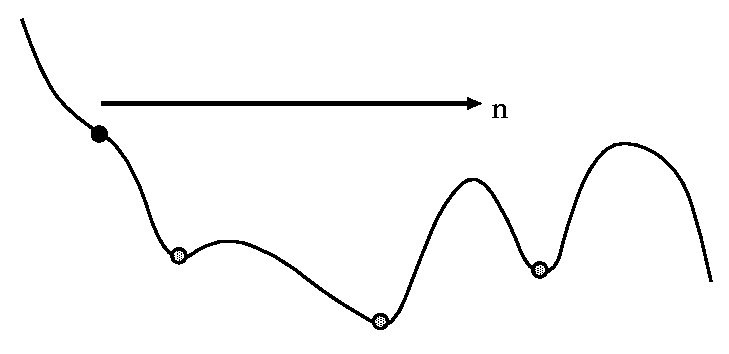
\includegraphics[width=0.6\textwidth]{linemin.eps}
\end{center}
\caption{
Figure for line minimization.
\label{fig:linmin}}
\end{figure}


In the first part of the line minimization routine the minimum is
bracketed, \ie we want a point $\a + s \nhat$ which has a lower
$\chi^2$ value than the points $\a + (s - ds) \nhat$
and $\a + (s + ds) \nhat$, where $ds$ is the step size.

When the line search routine is called, $ds = ds_i$.Here

\begin{eqnarray}
ds_i &=& {0.10 \chi^2 \over ||H||}
\end{eqnarray}

or equal to a value supplied by the user.


Steps with lengths $ds$ are taken along the direction $\nhat$ until
$\chi^2_{n-1} < \chi^2_{n}$, $n=1, \ldots$. If $\chi^2_{n-2} < \chi^2_{n-1}$,
\ie then the line search is restarted from $s=0$ with half the value of $ds$.

In the second part of the routine, a golden search is used to
narrow down the bracket triplet.




\begin{table}[!h]
\caption{
Sub-keywords for \textrm{prop} in table~\ref{tab:kw-sf}
concerning line minimization.
\label{tab:kw-lm-prop}
}
\begin{center}
\begin{tabular}{l|l}
\hline
\hline
\verb+ds_ini+       & Initial step size $ds_i$ when doing line minimization \\
                    & when fitting the properties parameters. \\
\hline
\hline
\end{tabular}
\end{center}
\end{table}


\begin{table}[!h]
\caption{
Sub-keywords for \textrm{pot} in table~\ref{tab:kw-sf}
concerning line minimization.
\label{tab:kw-lm-pot}
}
\begin{center}
\begin{tabular}{l|l}
\hline
\hline
\verb+ds_ini+       & Initial step size $ds_i$ when doing line minimization \\
                    & when fitting the potential parameters. \\
\hline
\hline
\end{tabular}
\end{center}
\end{table}













\subsection{Force calculation preliminaries}

Let the total potential energy of a system consisting of $N$ atoms be

\begin{equation}
V \equiv V(\rr_1, \ldots, \rr_N) = \sum_i V_i,
\end{equation}

where $V_i$ is the energy of atom $i$. The potential can be written
as a sum of $n$-body interactions:

\begin{equation}
V_i = \sum_j V^{(2)}_{ij}(\rr_i, \rr_j)
  + \sum_j \sum_k V^{(3)}_{ijk}(\rr_{ij}, \rr_{ik}, \rr_{jk})
  + \ldots
+ \left( \sum_{i_1} \ldots \sum_{i_M} \right) V^{(M-1)}_{i_1 \ldots i_M} + \ldots
\end{equation}

Here $V_{ij}$ is a pair potential, $V_{ijk}$ a three-body potential, and
$V_{i_1 \ldots i_M}$ is a general $M-1$-body interaction.


How do we calculate the force on any atom, say $v$ ? A fool-prof method is to
calculate the total derivative of the potential with respect to the
position $\rr_v$ of atom $v$:

\begin{eqnarray}
\F_v
  &=& - \nabla_{\rr_v} V \\
  &=& - \sum_{ij} \nabla_{\rr_v} V_{ij} - \sum_{ijk} \nabla_{\rr_v} V_{ijk} - \ldots \\
  &=& - \sum_{i} \nabla_{\rr_v} V_{iv} - \sum_{j} \nabla_{\rr_v} V_{vj} \nonumber \\
  & & - \sum_{ij} \nabla_{\rr_v} V_{ijv}  - \sum_{ik} \nabla_{\rr_v} V_{ivk} - \sum_{jk} \nabla_{\rr_v} V_{vjk} - \ldots \\
  &=& \sum_{i} \F_{iv} + \sum_{j} \F_{vj} \nonumber \\
  & & + \sum_{ij} \F_{ijv} + \sum_{ik} \F_{ivk} + \sum_{jk} \F_{vjk} + \ldots
\end{eqnarray}

Rewriting we have

\begin{eqnarray}
\F_v
  &=& \sum_{i} (\F_{iv} + \F_{vi} ) + \sum_{ij} (\F_{ijv} + \F_{ivj} + \F_{vij}) + \ldots
\label{eq:MD:F:atom}
\end{eqnarray}


\stars


If we have a pair potential, then the energy can be expressed as a function
of the distance $r_{ij}$ between atoms $i$ and $j$:

\begin{equation}
V = \sum_i \sum_j V_{ij}(r_{ij})
\end{equation}

and the total force on atom $v$ is

\begin{eqnarray}
\F_v &=& - \nabla_{\rr_v} \sum_j V_{vj} - \nabla_{\rr_v} \sum_i V_{iv} \\
  & \equiv & \sum_j \F_{v \Leftarrow j} + \sum_i \nabla_{\rr_i} \sum_i V_{iv} \\
  & \equiv & \sum_j \F_{v \Leftarrow j} - \sum_i \F_{i \Leftarrow v} \\
  &=& \sum_j \F_{v \Leftarrow j} + \sum_i \F_{v \Leftarrow i} \\
  &=& 2 \sum_j \F_{v \Leftarrow j},
\end{eqnarray}

where $\F_{v \Leftarrow j}$ is the force on atom $v$ due to interaction
with atom $j$. Here we used

\begin{eqnarray}
\nabla_{\rr_v} f(r_{iv})
  &=& - {\partial f(r_{iv}) \over \partial r_{iv}} {\rr_i - \rr_v \over r_{iv}} \\
  &=& - \nabla_{\rr_i} f(r_{iv}),
\end{eqnarray}



Hence we can use the following alternative method of calculating the force on any atom $v$:

\begin{eqnarray}
\F_v &=& \sum_{j=1, j \neq v}^N \F_{\v \Leftarrow j}, \\
\F_{\v \Leftarrow j} &=& - \sum_j \nabla_{\rr_v} V_{vj} = - {\partial V(r_{vj}) \over \partial r_{vj}} {\rr_v - \rr_j \over r_{vj}}, \\
\F_j &=& \F_j + (- \F_{v \Leftarrow j}), \quad j = 1, \ldots, N, j \neq v.
\end{eqnarray}

In summary: For the force on atom $v$ we use only the $V_{vj}$ term, and get the
contribution from $V_{jv}$ via Newton's third law when we calculate the
force on atom $j$.

\stars

Let's try the same thing with a three-body potential:


\begin{eqnarray}
V &=& \sum_i \sum_j \sum_k V_{ijk}(r_{ij}, r_{ik}, r_{jk}) \\
\F_v &=& \sum_j \sum_k \left(
  {\partial V_{vjk} \over \partial r_{vj}} {\rr_v - \rr_j \over r_{vj}}
+ {\partial V_{vjk} \over \partial r_{vk}} {\rr_v - \rr_k \over r_{vk}} \right) \\
  &=& \sum_j \sum_k \left( \F_{vj} + \F_{vk} \right) \\
\F_j &=& \F_j + (- \F_{v \Leftarrow j}), \\
\F_k &=& \F_k + (- \F_{v \Leftarrow k})
\end{eqnarray}


However, we are now missing terms that does not depend on the distances
$r_{vj}, r_{vk}, r_{jk}$ ! For instance, consider the cosine of the angle
between the bonds $\rr_v - \rr_j$ and $\rr_v - \rr_k$:

\begin{eqnarray}
\cos \theta_{vjk} &=& {(\rr_v - \rr_j) \cdot (\rr_v - \rr_k) \over r_{vj} r_{vk}}
\end{eqnarray}

It is not possible to differentiate this expression with respect to $r_{vj}, r_{vk}, r_{jk}$,
due to the scalar product in the numerator ! In this case we have to use the full
expression in Eq.~(\ref{eq:MD:F:atom}).







\subsection{Pressure calculation}

The pressure is calculated as

\begin{equation}
P = (N k_B T + W/3)/V,
\end{equation}

where $W$ is the virial:

\begin{equation}
W = - 3 V {\partial U \over \partial V}
\end{equation}

See Ref.~\cite{Koster-PRB62-2000,Beardmore-PRB60-1999}.

Writing

\begin{equation}
\rr_k = V^{1/3} \rho_k,
\end{equation}

where $\rho_k$ are dimensionless coordinates independent of the volume, we have

\begin{equation}
{\partial \over \partial V}
= \sum_k {\partial \rr_k \over \partial V} \cdot \nabla_{\rr_k}
= {1 \over 3} V^{-1} \sum_k V^{1/3} \rho_k \cdot \nabla_{\rr_k}
= {1 \over 3} V^{-1} \sum_k \rr_k \cdot \nabla_{\rr_k}
\end{equation}

so that

\begin{eqnarray}
W &=& - \sum_k \rr_k \cdot \nabla_{\rr_k} U
= - \sum_i \sum_{j, j\neq i} \sum_k \nabla_{\rr_k} U^{ij} \cdot \rr_k
\nonumber \\
  &=& \sum_i \sum_{j, j\neq i} \sum_k \F^{ij}_k \cdot \rr_k
\end{eqnarray}

For a pair potential:

\begin{eqnarray}
W &=& \sum_i \sum_{j, j\neq i} \sum_k \F^{ij}_k \cdot \rr_k
= \sum_i \sum_{j, j\neq i} \left( 
\F^{ij}_i \cdot \rr_i + \F^{ij}_j \cdot \rr_j
\right)
\nonumber \\
  &=& \sum_i \sum_{j, j\neq i} \left( 
\F^{ij}_i \cdot \rr_i - \F^{ij}_i \cdot \rr_j
\right)
\nonumber \\
  &=& \sum_i \sum_{j, j\neq i} \F^{ij}_i \cdot \rr_{ij}
\end{eqnarray}

For a many-body potential of the ABOP-form holds that

\begin{eqnarray}
\F^{ij}_i &=& - \sum_{k, k\neq i} \F^{ij}_k
\end{eqnarray}


Note:

\begin{eqnarray}
\sum_i \sum_{j, j\neq i} \sum_{k, k\neq i} \F^{ij}_k \cdot \rr_{ki}
&=&
\sum_i \sum_{j, j\neq i} \sum_{k, k\neq i} \F^{ij}_k \cdot \rr_k
-
\sum_i \sum_{j, j\neq i} \sum_{k, k\neq i} \F^{ij}_k \cdot \rr_i
\\
&=&
\sum_i \sum_{j, j\neq i} \sum_{k, k\neq i} \F^{ij}_k \cdot \rr_k
+
\sum_i \sum_{j, j\neq i} \F^{ij}_i \cdot \rr_i
\\
&=&
\sum_i \sum_{j, j\neq i} \sum_k \F^{ij}_k \cdot \rr_k
\end{eqnarray}

Therefore,

\begin{eqnarray}
W &=& \sum_i \sum_{j, j\neq i} \sum_{k, k\neq i} \F^{ij}_k \cdot \rr_{ki}
\end{eqnarray}









\subsection{Lennard-Jones potential}

The 6-12 Lennard-Jones potential gives the total energy of a dimer
with bond length $r_{ij}$  as

\begin{equation}
E_{dimer} = 4 \eps \left[
  \left({\sigma \over r_{ij}}\right)^{12}
- \left({\sigma \over r_{ij}}\right)^{6}
\right]
\label{eq:LJ}
\end{equation}

Here

\begin{equation}
r_{ij} = |\rr_i - \rr_j| = r_{ji}
\end{equation}



At equilibrium $E_{dimer} = -\eps$, making the energy per atom, \ie
the cohesive energy $E_c$, $-\eps/2$.
By definition,

\begin{equation}
E_c = {1 \over N} \sum_i \sum_j E_{ij},
\end{equation}

Here $E_{ij}$ is the energy contribution to atom $i$
due to neighbor $j$. Putting

\begin{equation}
E_{ij} = A E_{dimer}
\end{equation}

we get from the cohesive energy equation that

\begin{equation}
-\eps = A (-2\eps)
\end{equation}

so that $A=1/2$. This means that

\begin{equation}
E_{ij} = 2 \eps \left[
  \left({\sigma \over r_{ij}}\right)^{12}
- \left({\sigma \over r_{ij}}\right)^{6}
\right]
\end{equation}

in the formula

\begin{equation}
E = \sum_{i=1}^N \sum_{j, j\neq i}^N E_{ij}
\end{equation}

for the energy of an atom system.

The force on atom $i$ is

\begin{equation}
\F_{ij} = 
- 12 \eps \left[
 2 \left( {\sigma \over r_{ij}} \right)^{12}
-  \left( {\sigma \over r_{ij}} \right)^6
\right]
{\rr_i - \rr_j \over r^2_{ij}}
\end{equation}









\subsection{Morse potential}

The Morse potential gives the total energy of a dimer as

\begin{equation}
E_{dimer} = D \left[
e^{-2\beta(r_{ij}-r_0)} - 2 e^{-\beta(r_{ij}-r_0)]}
\right]
\label{eq:morse}
\end{equation}

At equilbrium, $r_{ij} = r_0$,

\begin{equation}
E_{dimer} = -D
\end{equation}

Cohesive energy is then $E_c = -D/2$. As above, we obtain

\begin{equation}
E_{ij}
= {1 \over 2} D \left[
e^{-2\beta(r_{ij}-r_0)} - 2 e^{-\beta(r_{ij}-r_0)]}
\right]
\end{equation}

We now have

\begin{equation}
\F_{ij}
= - D \beta  \left[
e^{-2\beta(r_{ij}-r_0)} - e^{-\beta(r_{ij}-r_0)]}
\right]
{\rr_i - \rr_j \over r_{ij}}
\end{equation}



\stars

Some essential derivatives are:

\begin{eqnarray}
\nabla_i V_{R,ij} &=& - {D_0 \beta \sqrt{2S} \over S-1} 
\exp\left[ - \beta \sqrt{2S} (r_{ij} -r_{0,ij}) \right] {\rr_i - \rr_j \over r_{ij}}
\\
\nabla_i V_{A,ij} &=& - {S D_0 \beta \sqrt{2/S} \over S-1}
\exp\left[ - \beta \sqrt{2/S} (r_{ij} -r_{0,ij}) \right] {\rr_i - \rr_j \over r_{ij}}
\\
\nabla_i f_{C,ij} &=& {\rr_i - \rr_j \over r_{ij}}
\left\{
\begin{array}{ll}
0,                   & r \leq R - D, \\
-{\pi \over 4 D} \cos \left( {\pi \over 2} {r_{ij} - R \over D} \right), & |R - r_{ij}| < D  \\
0,                   & r \geq R + D
\end{array}
\right.
\\
\nabla_i b_{ij}
 &=& - {1 \over 2 (1 + \chi_{ij})^{3/2}} \nabla_{\rr_i} \chi_{ij} \\
\nabla_i \chi_{ij}
  &=&
  \sum_{k, k \neq i, k \neq j} (\nabla_{\rr_i} f_{C,ik}) g_{ijk} \omega_{ijk} \exp\left[
  \alpha_{ijk}(r_{ij} - r_{ik}) \right] \nonumber \\
  & &
+ \sum_{k, k \neq i, k \neq j} f_{C,ik} (\nabla_{\rr_i} g_{ijk}) \omega_{ijk} \exp\left[
  \alpha_{ijk}(r_{ij} - r_{ik}) \right]  \nonumber \\
  & &
+ \sum_{k, k \neq i, k \neq j} f_{C,ik} g_{ijk} \omega_{ijk} \nabla_{\rr_i} \exp\left[
  \alpha_{ijk}(r_{ij} - r_{ik}) \right]
\\
\nabla_i g_{ijk}
  &=& \gamma {c^2 \over (d^2 + (h + \cos \theta_{ijk})^2)^2} 2 (h + \cos \theta_{ijk})
\nabla_i \cos \theta_{ijk}
\end{eqnarray}

and

\begin{eqnarray}
\nabla_i \cos \theta_{ijk}
  &=& \nabla_i { (\rr_j - \rr_i) \cdot (\rr_k - \rr_i) \over r_{ij} r_{ik}} \\
  &=&
\nabla_i { \rr_j \cdot \rr_k - \rr_j \cdot \rr_i - \rr_i \cdot \rr_k + r_i^2
\over r_{ij} r_{ik} } \\
  &=&
{1 \over r_{ij} r_{ik} }
( - \rr_j - \rr_k + 2 \rr_i )
\nonumber \\
  & &
- {\cos \theta_{ijk} \over r_{ij}} {\rr_i - \rr_j \over r_{ij}}
- {\cos \theta_{ijk} \over r_{ik}} {\rr_i - \rr_k \over r_{ik}}
\nonumber \\
  &=&
  (\rr_i - \rr_j) \left[
  {1 \over r_{ij} r_{ik} }
- {\cos \theta_{ijk} \over r^2_{ij}}
\right]
\nonumber \\
  & &
 +(\rr_i - \rr_k) \left[
  {1 \over r_{ij} r_{ik} }
- {\cos \theta_{ijk} \over r^2_{ik}}
\right]
\end{eqnarray}

and also

\begin{eqnarray}
  & & \nabla_{\rr_i} \exp\left[ \alpha_{ijk}(r_{ij} - r_{ik}) \right] \\
  &=&
{ \rr_i - \rr_j \over r_{ij}} \alpha_{ijk} \exp\left[ \alpha_{ijk}(r_{ij} - r_{ik}) \right]
-
{ \rr_i - \rr_k \over r_{ik}} \alpha_{ijk} \exp\left[ \alpha_{ijk}(r_{ij} - r_{ik}) \right]
\end{eqnarray}




With

\begin{equation}
V = {1 \over 2} \sum_i \sum_{j} f_{C,ij} \left( V_{R,ij} - b_{ij} V_{A,ij} \right)
\end{equation}

the force on atom $v$ is

\begin{eqnarray}
\F_v &=&
      - {1 \over 2} \sum_j (\nabla_v f_{C,vj}) \left( V_{R,vj} - b_{vj} V_{A,vj} \right)
\nonumber \\
  & & - {1 \over 2} \sum_j (\nabla_v f_{C,jv}) \left( V_{R,jv} - b_{jv} V_{A,jv} \right)
\nonumber \\
  & & - {1 \over 2} \sum_j f_{C,vj} \left( (\nabla_v V_{R,vj}) - b_{vj} (\nabla_v V_{A,vj})
- (\nabla_v b_{vj}) V_{A,vj} \right)
\nonumber \\
  & & - {1 \over 2} \sum_j f_{C,jv} \left( (\nabla_v V_{R,jv}) - b_{jv} (\nabla_v V_{A,jv})
- (\nabla_v b_{jv}) V_{A,jv} \right)
\nonumber \\
  & & + {1 \over 2} \sum_i \sum_j f_{C,ij} (\nabla_v b_{ij}) V_{A,ij}
\\
  &=& - {1 \over 2} \sum_j (\nabla_v f_{C,vj}) \left( V_{R,vj} - b_{vj} V_{A,vj} \right)
\nonumber \\
  & & - {1 \over 2} \sum_j (\nabla_v f_{C,jv}) \left( V_{R,jv} - b_{jv} V_{A,jv} \right)
\nonumber \\
  & & - {1 \over 2} \sum_j f_{C,vj} \left( (\nabla_v V_{R,vj}) - b_{vj} (\nabla_v V_{A,vj})\right)
\nonumber \\
  & & - {1 \over 2} \sum_j f_{C,jv} \left( (\nabla_v V_{R,jv}) - b_{jv} (\nabla_v V_{A,jv})\right)
\nonumber \\
  & & + {1 \over 2} \sum_j (\nabla_v b_{vj}) V_{A,vj}
\nonumber \\
  & & + {1 \over 2} \sum_j (\nabla_v b_{jv}) V_{A,jv}
\nonumber \\
  & & + {1 \over 2} \sum_i \sum_j f_{C,ij} (\nabla_v b_{ij}) V_{A,ij}
\end{eqnarray}

Notice the last term in this expression. It is crucial.
Notice also that it is added only when $i \neq v \neq j$, \ie for atom $k$ in the sum for $b_{ij}$.


\stars


\begin{eqnarray}
W &=& \sum_i \sum_{j, j\neq i} \sum_{k, k\neq i} \F^{ij}_k \cdot \rr_{ki},
\end{eqnarray}

where

\begin{eqnarray}
\sum_{k, k\neq i} \F^{ij}_k \cdot \rr_{ki}
  &=&
- \nabla_{\rr_j} \left[ f_c(r_{ij}) V_R(r_{ij}) - b_{ij} f_c(r_{ij}) V_A(r_{ij}) \right] \cdot \rr_{ji}
\nonumber \\
  & &
+ f_c(r_{ij}) V_A(r_{ij}) \sum_{k, k\neq i,j} \nabla_{\rr_k} b_{ij} \cdot \rr_{ki}
\end{eqnarray}

Note: Earlier we had derivatives with respect to $\rr_{i}$. The current derivatives of $b_{ij}$
will be different !!!


\begin{eqnarray}
\nabla_j \chi_{ij}
  &=&
  \sum_{k, k \neq i, k \neq j} f_{C,ik} (\nabla_{\rr_j} g_{ijk}) \omega_{ijk} \exp\left[
  \alpha_{ijk}(r_{ij} - r_{ik}) \right]  \nonumber \\
  & &
+ \sum_{k, k \neq i, k \neq j} f_{C,ik} g_{ijk} \omega_{ijk} \nabla_{\rr_j} \exp\left[
  \alpha_{ijk}(r_{ij} - r_{ik}) \right]
\end{eqnarray}


\begin{eqnarray}
\nabla_j \cos \theta_{ijk}
  &=& \nabla_j { (\rr_j - \rr_i) \cdot (\rr_k - \rr_i) \over r_{ij} r_{ik}} \\
  &=&
\nabla_j { \rr_j \cdot \rr_k - \rr_j \cdot \rr_i - \rr_i \cdot \rr_k + r_i^2
\over r_{ij} r_{ik} } \\
  &=&
{- \rr_{ik} \over r_{ij} r_{ik} }
- 
{ \rr_{ij} \cdot \rr_{ik} \over r_{ij}^2 r_{ik}} \left( -{\rr_{ij} \over r_{ij}} \right) \\
  &=&
{- \rr_{ik} \over r_{ij} r_{ik} }
- 
{ \cos \theta_{ijk} \over r_{ij}} \left( -{\rr_{ij} \over r_{ij}} \right) \\
  &=&
{1 \over r_{ij} r_{ik}}
\left[
- \rr_{ik} + \cos \theta_{ijk} r_{ik} {\rr_{ij} \over r_{ij}}
\right]
\\
  &=& 
{1 \over r_{ij}}
\left[
- {\rr_{ik} \over r_{ik}}
+ \cos \theta_{ijk} {\rr_{ij} \over r_{ij}}
\right]
\end{eqnarray}



\begin{eqnarray}
\nabla_k \cos \theta_{ijk}
  &=& \nabla_k { (\rr_j - \rr_i) \cdot (\rr_k - \rr_i) \over r_{ij} r_{ik}} \\
  &=&
\nabla_k { \rr_j \cdot \rr_k - \rr_j \cdot \rr_i - \rr_i \cdot \rr_k + r_i^2
\over r_{ij} r_{ik} } \\
  &=&
{\rr_j - \rr_i \over r_{ij} r_{ik}}
+
{\rr_{ji} \cdot \rr_{ki} \over r_{ik}^2 r_{ij}} {\rr_{ik} \over r_{ik}}
\\
  &=&
{- \rr_{ij} \over r_{ij} r_{ik}}
+
\cos \theta_{ijk} {\rr_{ik} \over r_{ik}^2}
\end{eqnarray}



When \eg only $d$-band contributes to the energy, then the force on atom $v$ is

\begin{eqnarray}
\F_v
  &=&
- {1 \over 2} \nabla_v \sum_i \sum_j V_{2,ij}
- \nabla_v \sum_i F_{d,i}(\rho^a_{i})
\nonumber \\
  &=&
- {1 \over 2} \nabla_v \sum_j V_{2,vj}
- \nabla_v \sum_i F_{d,i}(\sum_j \rho_{ij}(r_{ij})) \nonumber \\
  &=&
- {1 \over 2} \nabla_v \sum_j V_{2,vj}
\nonumber \\
  & &
- {\partial F_{d,v}(\rho^a_v) \over \partial \rho^a_v} \sum_j {\partial \rho^a_v \over \partial r_{vj}} {\rr_v - \rr_j \over r_{vj}}
\nonumber \\
  & &
+ \sum_j  {\partial F_{d,j}(\rho^a_j) \over \partial \rho^a_j} {\partial \rho^a_j \over \partial r_{jv}} {\rr_j - \rr_v \over r_{jv}}
\nonumber \\
  &=&
- {1 \over 2} \nabla_v \sum_j V_{2,vj} \nonumber \\
  & &
- \sum_j  \left(
  {\partial F_{d,v}(\rho^a_v) \over \partial \rho^a_v}
+ {\partial F_{d,j}(\rho^a_j) \over \partial \rho^a_j}
\right)
{\partial \rho^a_j \over \partial r_{vj     }} {\rr_v - \rr_j \over r_{vj}}
\end{eqnarray}

